%! Author = joels
%! Date = 05/01/2021

\section{Architektur und fortgeschrittene Themen}
\subsection{Architektur}
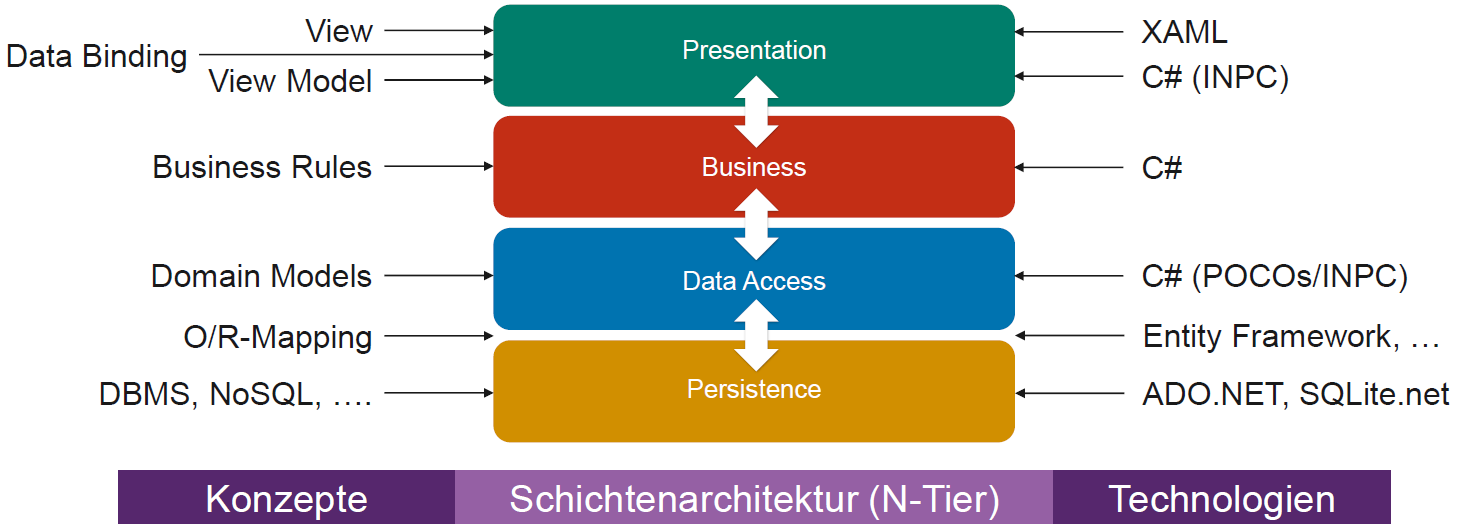
\includegraphics{architektur.png}
\textbf{\textcolor{blue}{Hauptgründe für Schichten:}}
\begin{itemize}[topsep=0pt, leftmargin=4mm]
    \setlength\itemsep{-0.3em}
    \item Fachliche, technische oder organisatorische Grenzen
    \item Positiver Einfluss auf SW-Qualitätsmerkmale
    \item Sorgen bei grossen Projekt für Überblick
\end{itemize}
\subsubsection{Horizontale und vertikale Schnitte}
\textbf{\textcolor{blue}{Horizontale Schnitte:}}
\begin{itemize}[topsep=0pt, leftmargin=4mm]
    \setlength\itemsep{-0.3em}
    \item Traditioneller Ansatz
    \item Geeignet für \dq Technologie Teams\dq
    \item Austausch von Technologien einfacher
\end{itemize}
\textbf{\textcolor{blue}{Horizontale Schnitte:}}
\begin{itemize}[topsep=0pt, leftmargin=4mm]
    \setlength\itemsep{-0.3em}
    \item Modernerer Ansatz
    \item Geeignet für \dq Feature Teams\dq
    \item Austausch von Technologien schwieriger
\end{itemize}
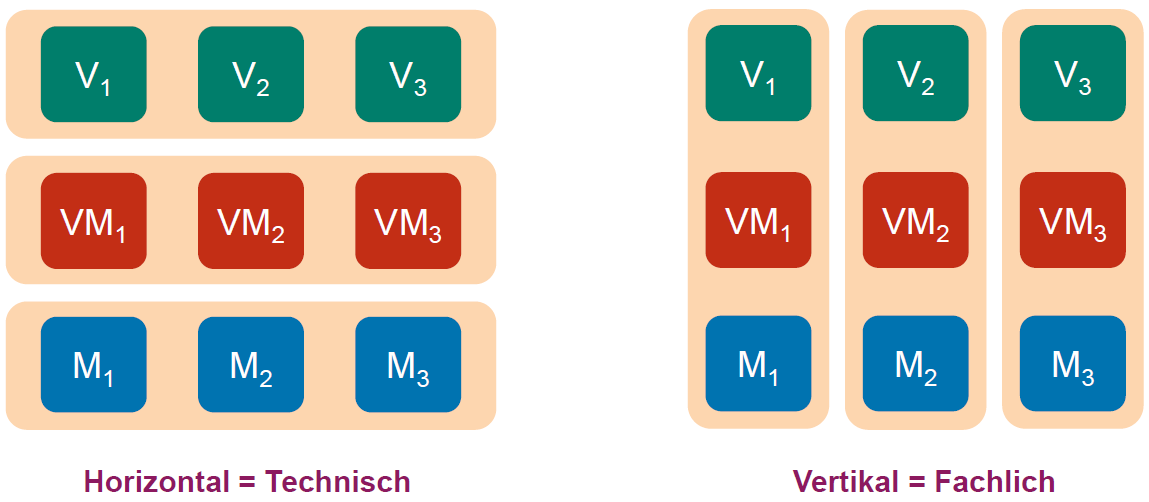
\includegraphics{architektur_schnitte.png}
\subsubsection{Dependency Injection}
\begin{itemize}[topsep=0pt, leftmargin=4mm]
    \setlength\itemsep{-0.3em}
    \item Client kennt Service nur als Interface
    \item Injector erzeugt Service und Client
    \item Injector injiziert Abhängigkeiten via: Konstruktor, Methode, property
\end{itemize}
\begin{center}
    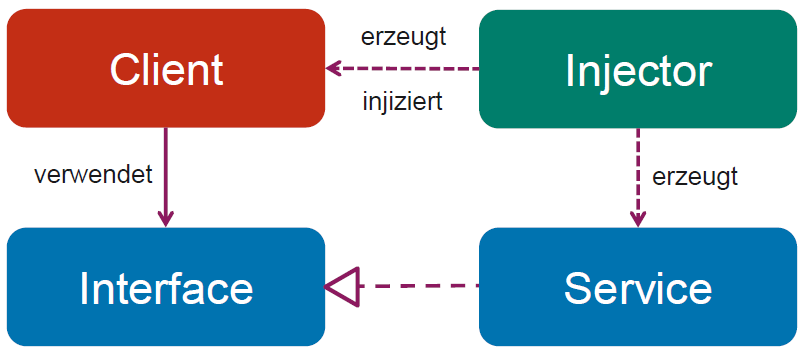
\includegraphics[width=0.7\linewidth]{dependency_injection.png}
\end{center}
\subsubsection{Grundmuster für DI}
\begin{itemize}[topsep=0pt, leftmargin=4mm]
    \setlength\itemsep{-0.3em}
    \item 1. Interface für Verhalten definieren
    \item 2. Interface im View Model verwenden
    \item 3. Interface im Plattform-Projekt implementieren
    \item 4. Service im Plattform-Projekt erzeugen
    \item 5. View Model im Plattform-Projekt erzeugen
    \item 6. Service in View Model injizieren
\end{itemize}
\begin{center}
    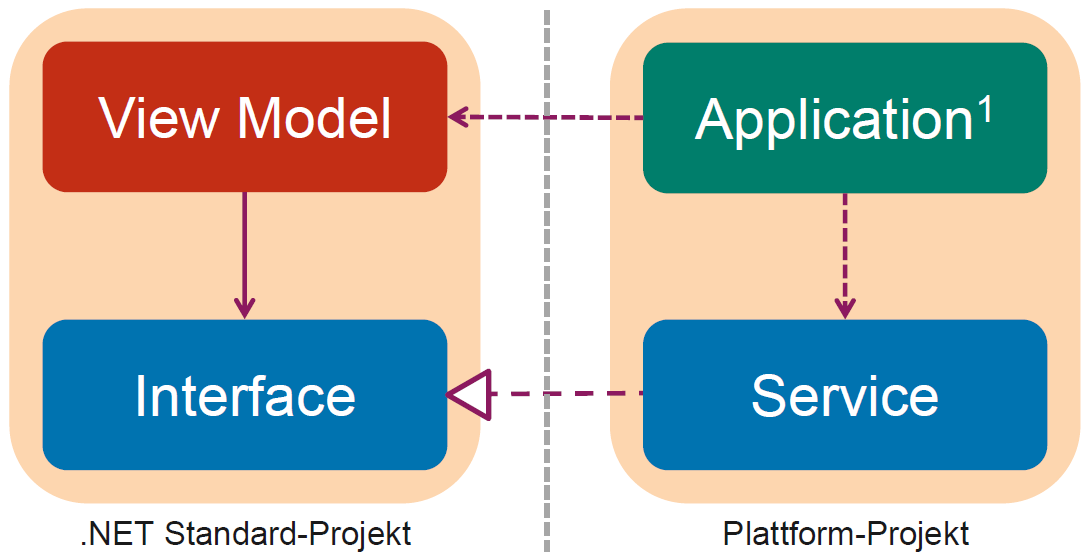
\includegraphics[width=0.7\linewidth]{dependency_injection_grundmuster.png}
\end{center}
\subsubsection{Vor- und Nachteile von DI}
\textbf{\textcolor{blue}{Vorteile:}}
\begin{itemize}[topsep=0pt, leftmargin=4mm]
    \setlength\itemsep{-0.3em}
    \item Geringere Kopplung zwischen Klassen
    \item Zwang zur Separation of Concerns
    \item Austauschbarkeit von Services
    \item Erhöhte Testbarkeit
    \item Weniger Glue Code im Client
\end{itemize}
\textbf{\textcolor{blue}{nachteile:}}
\begin{itemize}[topsep=0pt, leftmargin=4mm]
    \setlength\itemsep{-0.3em}
    \item Zusätzliche Komplexität
    \item Erschwertes Debugging
    \item Parameterlisten bei vielen Abhängigkeiten
    \item Mehr Glue Code beim Injector
\end{itemize}
\subsection{Mehrsprachigkeit}
\subsubsection{Mehrsprachigkeit mit Resources}
\begin{itemize}[topsep=0pt, leftmargin=4mm]
    \setlength\itemsep{-0.3em}
    \item Strings in Resource Dictionaries
    \item Pro Sprache eine XAML-Datei
    \item Zugriff im XAML über \textcolor{blue}{{DynamicResource ... }}
    \item Zugriff in C\# über \textcolor{blue}{FindResource()}
    \item Anpassen der Resource Dictionaries bei Sprachänderung im Code Behind
\end{itemize}
\begin{lstlisting}
// Übersetzungen
<ResourceDictionary>
    <system:String x:Key="Key1">Translation 1</system:String>
</ResourceDictionary>

// XAML
<Window>
    <Label Content="{DynamicResource Key1}" />
</Window>

// Code Behind
public void LoadTranslations(string key) {
    var uri = new Uri($"/MyApp;component/Trans.{key}.xaml",
    UriKind.RelativeOrAbsolute);
    var rd = new ResourceDictionary { Source = uri };
    foreach (var rdKey in rd.Keys) {
        Resources[rdKey] = rd[rdKey];
    }
}
\end{lstlisting}
\subsubsection{Mehrsprachigkeit mit RESX}
\begin{itemize}[topsep=0pt, leftmargin=4mm]
    \setlength\itemsep{-0.3em}
    \item Strings in RESX-Dateien
    \item Pro Sprache eine RESX-Datei
    \item Zugriff im XAML über \textcolor{blue}{{x:Static ... }}
    \item Zugriff in C\# über generierte Klasse
    \item Anpassen der \dq Culture\dq bei Sprachänderung in beliebigen C\# Code
\end{itemize}
\begin{lstlisting}
// Übersetzungen
<?xml version="1.0" encoding="utf-8"?>
<root>
    <data name="Key1" xml:space="preserve">
        <value>Translation 1</value>
    </data>
</root>

// XAML
<Window xmlns:t="clr-namespace:MyApp.Translations">
    <Label Content="{x:Static t:Translations.Key1}" />
</Window>

// Code Behind
public void LoadTranslations(string key) {
    // Key kann z.B. "de" oder "en-US" sein
    Translations.Culture = new CultureInfo(key);
}
\end{lstlisting}
\subsubsection{Mehrsprachigkeit Gedanken}
Für Zugriff im C\#-Code einen Translation Service benutzten. Dadurch bleibt Code unabhängig von einem konktreten Übersetzungsmechanismus. Dies eröffnet die Möglichkeit, Übersetzungen als Properties auf dem View Model zu halten.

\subsection{Routed Events}
\begin{itemize}[topsep=0pt, leftmargin=4mm]
    \setlength\itemsep{-0.3em}
    \item UI Ereignisse, auf die reagiert werden kann
    \begin{itemize}[topsep=0pt, leftmargin=4mm]
        \setlength\itemsep{-0.3em}
        \item Maustaste wurde gedrückt
        \item Maus wurde bewegt
        \item Taste auf Tastatur wurde gedrückt
        \item etc.
    \end{itemize}
    \item Bewegen sich in zwei Phasen durch den Visual Tree
    \begin{itemize}[topsep=0pt, leftmargin=4mm]
        \setlength\itemsep{-0.3em}
        \item Tunneling – Abwärts bis zum fokussierten Element
        \item Bubbeling – Aufwärts vom fokussierten Element
    \end{itemize}
    \item Bewegung kann von jedem Element gestoppt werden: Setzen von RoutedEventArgs.Handled auf false
\end{itemize}
\subsubsection{Tastatureingabe}
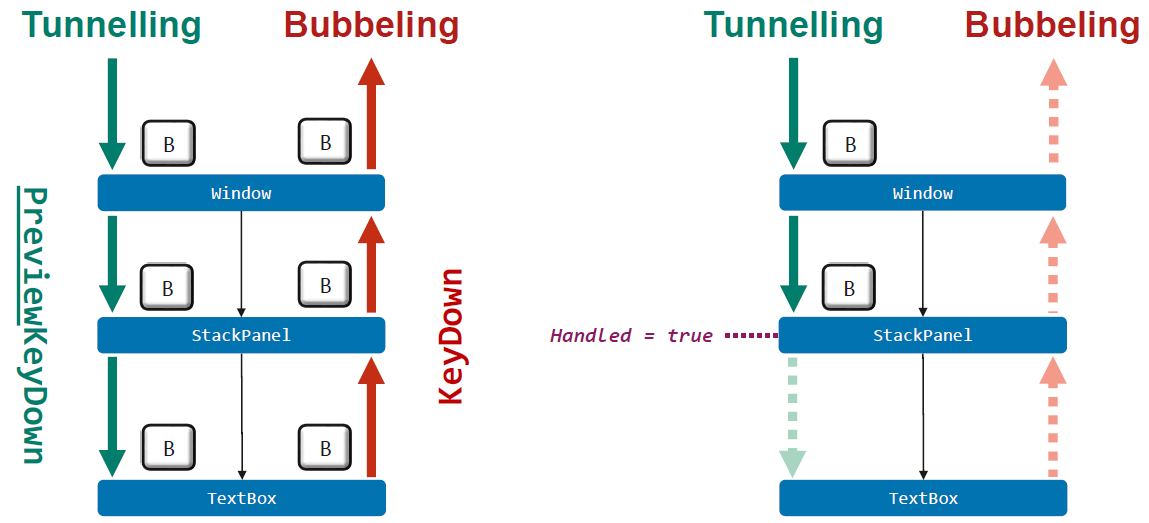
\includegraphics{routed_events.png}
\begin{lstlisting}
// XAML
<Window PreviewKeyDown="Window_OnPreviewKeyDown"
    KeyDown="Window_OnKeyDown">
  <StackPanel PreviewKeyDown="StackPanel_OnPreviewKeyDown"
      KeyDown="StackPanel_OnKeyDown">
    <TextBox PreviewKeyDown="TextBox_OnPreviewKeyDown"
        KeyDown="TextBox_OnKeyDown" />
  </StackPanel>
</Window>

// Code Behind
private void Window_OnPreviewKeyDown(object sender, KeyEventArgs e) { ... }
private void StackPanel_OnPreviewKeyDown(object sender, KeyEventArgs e) { ... }
private void TextBox_OnPreviewKeyDown(object sender, KeyEventArgs e) { ... }
\end{lstlisting}
\subsection{Background Execution}
\subsubsection{WPF Threading Model}
\textbf{In jeder WPF-Applikation gibt es mindestens zwei Threads.}\\
\textbf{UI Thread:} Verwaltet UI, empfängt Ereignisse und führt Aktionen aus.\\
\textbf{Rendering Thread:} Läuft im Hintergrund, zeichnet Controls auf den Screen.\\
$\rightarrow$ Dadurch werden Controls auch dann neu gezeichnet, wenn der UI Thread blockiert ist
\subsubsection{Mechanismen}
.NET kennt verschiedene Mechanismen für Backgrounding.
\begin{itemize}[topsep=0pt, leftmargin=4mm]
    \setlength\itemsep{-0.3em}
    \item Klasse Task (Einfaches Konzept)
    \item Keywords async/await (In modernen Apps verwendet)
    \item Parallel LINQ (PLINQ)
\end{itemize}
\begin{lstlisting}
Task.Run(() => {
    // Ausführung auf Background Thread
    // Operationen laufen parallel zum UI Thread
});
// UI-Thread läuft hier weiter. Nur er darf das UI verändern
\end{lstlisting}
\subsubsection{Dispatcher}
Erlaubt priorisiertes Abarbeiten von Aufgaben in einem Thread. Delegieren von Aufgaben an den Dispatcher:\\
\textcolor{blue}{Invoke()} - Synchron, Aufrufer läuft erst nach Abarbeitung der Aufgabe weiter\\
\textcolor{blue}{BeginInvoke()} - Asynchron, Aufrufer läuft parallel zur Aufgabe weiter
\begin{lstlisting}
// IsCalculating ist ein ViewModel-Property
IsCalculating = true;
Task.Run(() => {
    // Kein Dispatcher.Invoke(...) nötig
    IsCalculating = false;
});

// Einmalige Initialisierung in Application.OnStartup():
// RelayCommand.Dispatch = Dispatcher.Invoke;
public sealed class RelayCommand : ICommand {
    public static Action<Action> Dispatch { get; set; }
    public void RaiseCanExecuteChanged() {
        Dispatch(() => CanExecuteChanged?.Invoke(this, EventArgs.Empty));
    }
}
\end{lstlisting}